\documentclass{article}
\usepackage[sc]{mathpazo}
\linespread{1.15}  
% \usepackage[T1]{fontenc}
%\usepackage[T1]{fontenc}
%\usepackage[sfdefault,scaled=.85]{FiraSans}
%\usepackage{newtxsf}
%\usepackage{mathptmx}
%\usepackage[T1]{fontenc}
%\usepackage{sansmathfonts} 
%\renewcommand*\familydefault{\sfdefault} %% Only if the base font of the document is to be sans serif  
\usepackage[utf8]{inputenc}
\usepackage[margin=2cm]{geometry}
\usepackage{fullpage,enumitem,amssymb,amsmath,tikz,pgfplots,xcolor,cancel,gensymb,hyperref,graphicx,physics,tcolorbox}
\usepackage{indentfirst}
\setlength{\parindent}{0em}
\graphicspath{{./images/}}

\title{A Module on the Maths behind Q6-7}
\author{Chris Wang}
\date{\today}

\begin{document}
\maketitle

\textit{Note: Practice questions are denoted by a blue box. There are three practice questions in this module; you are only required to do one. Animations are denoted by a red box. Sections that are labeled with ``enrichment'' are completely optional. Additionally, please answer the survey question immediately below.}

\begin{tcolorbox}[arc=2mm, colback=green!10!white, colframe=green!50!black, title=\textsc{Survey Question}]
	After reading the module and doing the associated activities, summarize, in one to two sentences, the most important concept you learned through the module. If you have already seen everything in this module before, ``nothing'' is also a valid answer. Additionally, if anything was particularly confusing, please make a note of it here too.
\end{tcolorbox}

% \section*{Alternative Coordinates}

% In Q6, you encountered the Stern-Gerlach experiment and the physical realness of intrinsic electron spin. You may also have noticed that we used angular arguments, such as $\theta$, to describe the orientation of an electron with respect to the magnetic field. This is due to the convenience of using alternative coordinate systems to represent the orientation of the electron. In this section, we'll discuss a few types of coordinate systems most commonly used in physics. I will assume you know Cartesian coordinates fairly well, so I will mostly be discussing polar, cylindrical, and spherical coordinates. Let's first begin with a brief review on vectors.

% \vspace{1em}

% \begin{tcolorbox}[arc=2mm, colback=white]

%     \subsection*{A Brief Review on Vectors}
    
%     Vectors are mathematical objects that carry two pieces of information to uniquely identify itself: a \textbf{magnitude} and \textbf{direction}. In Q6, the spin vector described the magnitude of an electron's spin and the direction it was pointing relative to the magnetic field. For a three-component vector, which can be denoted either as $\vec{v}$ or $\mathbf{v}$, the magnitude of the vector is given by:
%     \[
%     v=|\vec{v}| = |\mathbf{v}| = \sqrt{v_x^2 + v_y^2 + v_z^2},
%     \]
%     where $v_x$, $v_y$, and $v_z$ are the components of the vector in the $x$, $y$, and $z$ directions, respectively. Given two vectors $\vec{v}$ and $\vec{w}$, we can also add or subtract them component-wise:
%     \[
%     (\vec{v} + \vec{w})^\intercal = \begin{bmatrix}
%     v_x + w_x & 
%     v_y + w_y &
%     v_z + w_z
%     \end{bmatrix}
%     \]
% \end{tcolorbox}

% \begin{tcolorbox}[arc=2mm, colback=magenta!15!white, colframe=magenta!80!black, title=\textsc{Vector Norms and Products (Enrichment)}]
%     The magnitude of a vector presented above is also known as the 2-norm of a vector. There are other types of norms that can be used for various other purposes. For instance, the 1-norm of a vector, which is also known as the Manhattan norm, is given by:
%     \[
%     \|\vec{v}\|_1 = |v_x| + |v_y| + |v_z|.
%     \]
%     As its name suggests, we can use it to find the distance between two points given the constraint that we have to travel along a grid, much like how the streets of Manhattan are laid out. The above cases are special cases of something called the $p$-norm, which is given by:
%     \[
%     \|\vec{v}\|_p = \left(|v_x|^p + |v_y|^p + |v_z|^p\right)^{1/p}.
%     \]
%     Now we discuss vector products, which come up frequently in physics. 
    
%     \begin{tcolorbox}[arc=2mm,colback=white]
%     If we have two vectors $\vec{v}$ and $\vec{w}$, we can take their dot product, which is given by:
%     \[
%     \vec{v} \cdot \vec{w} = v_x w_x + v_y w_y + v_z w_z.
%     \]
%     The dot product is a scalar quantity that tells us, approximately, how ``similar'' or ``parallel'' two vectors are. In fact, we use the dot product to find the angle between two vectors and the projection of one vector onto another. The angle, $\theta$, between two vectors is given by:
%     \[
%     \cos(\theta) = \frac{\vec{v} \cdot \vec{w}}{|\vec{v}||\vec{w}|}.
%     \]
%     \end{tcolorbox}
%     If we wanted to project one vector $\vec{v}$ onto another vector $\vec{w}$, we can do so:
%     \[
%     \text{proj}_{\vec{w}}(\vec{v}) = \frac{\vec{v} \cdot \vec{w}}{|\vec{w}|^2}\vec{w}.
%     \]
%     These quantities are maximized when the two vectors are parallel, giving us a sense of how similar the two vectors are. The cross product of two vectors, $\vec{v} \times \vec{w}$, is another vector product. However, the cross product is a \textit{vector}, and it is perpendicular to both $\vec{v}$ and $\vec{w}$. It is given by:
%     \[
%     \vec{v} \times \vec{w} = \begin{bmatrix}
%     v_y w_z - v_z w_y \\
%     v_z w_x - v_x w_z \\
%     v_x w_y - v_y w_x
%     \end{bmatrix}.
%     \]
% \end{tcolorbox}

% \subsection*{Polar and Cylindrical Coordinates}
%     Polar coordinates are an alternative coordinate system in two dimensions. Instead of using $x$ and $y$ coordinates, we use a distance $r$ from the origin and an angle $\theta$ from the $x$-axis. The conversion between Cartesian and polar coordinates is given by:
%     \[
%     \begin{aligned}
%     x &= r\cos(\theta) \\
%     y &= r\sin(\theta)
%     \end{aligned}
%     \quad \longleftrightarrow \quad
%     \begin{aligned}
%     r &= \sqrt{x^2 + y^2} \\
%     \theta &= \tan^{-1}\left(\frac{y}{x}\right).
%     \end{aligned}
%     \]
%     This coordinate system is particularly useful when we deal with circular or radial motion (for instance, the top-down view of the electron's procession as viewed from the $+z$ axis). The distance $r$ is the magnitude of the vector, while the angle $\theta$ is the direction. The angle $\theta$ is measured in radians, which is a unit of angle that is defined as the arc length of a circle divided by the radius of the circle. Therefore, there are $2\pi$ radians in a full circle. 

%     \vspace{1em}

%     Cylindrical coordinates are almost identical to polar coordinates, except cylindrical coordinates operate in three dimensions. The $x$ and $y$ transformations are identical, while the $z$ transformation is simply the $z$ coordinate. You may encounter some problems in Mechanics or Electromagnetism that are easier to solve in cylindrical coordinates, such as solving for the equation of motion for a bead sliding on a helical wire. 

% \subsection*{Spherical Coordinates}

%     Spherical coordinates are another alternative coordinate system that is used in three dimensions. Instead of using $x$, $y$, and $z$ coordinates, we use a distance $r$ from the origin, an angle $\theta$ from the $z$-axis, and an angle $\phi$ from the $x$-axis. The conversion between Cartesian and spherical coordinates is given by:
%     \[
%     \begin{aligned}
%     x &= r\sin(\theta)\cos(\phi) \\
%     y &= r\sin(\theta)\sin(\phi) \\
%     z &= r\cos(\theta)
%     \end{aligned}
%     \quad \longleftrightarrow \quad
%     \begin{aligned}
%     r &= \sqrt{x^2 + y^2 + z^2} \\
%     \theta &= \cos^{-1}\left(z / r\right) \\
%     \phi &= \tan^{-1}\left(y / x\right).
%     \end{aligned}
%     \]
%     Beware of the rather confusing notation: $\theta$ now denotes the angular separation between a vector in three-dimensional space, or $\mathbb{R}^3$, and the $z$-axis. Meanwhile, $\phi$ denotes the angle in the $xy$-plane. These angles have special names: $\theta$ is the \textbf{polar} angle, while $\phi$ is the \textbf{azimuthal} angle. Let's have a look at how these coordinates can be visualized in the following animation. 

%     \begin{tcolorbox}[arc=2mm, colback=red!10!white, colframe=red!50!black, title=\textbf{ACTIVITY}]
%         Watch the animation $\rightarrow$ \textcolor{red}{\href{https://youtu.be/S4nlCkDcxQs}{here}}, which illustrates spherical coordinates in more detail.
%     \end{tcolorbox}

%     \begin{tcolorbox}[colframe=blue!50!black, arc=2mm, title=\textsc{Practice 1}]
%         Consider the case of the precessing electron in Figure Q6.5. Supposing the electron precesses at an angular velocity of $\omega$, express the electron's spin vector in spherical coordinates. \textit{Hint: express the angle between the spin vector and the $z$-axis as $\theta$ and use boundary conditions to derive the time-dependence of the $x$ and $y$ coordinates.}
%     \end{tcolorbox}

\section*{A Whiff of Linear Algebra}

    In Q7, you encountered the beginnings of Dirac's bra-ket notation for quantum mechanics. To briefly review, recall the notion of a \textbf{q-vector} for \textbf{bras} and \textbf{kets}:
    \[
    \text{A ket is }\ket{\psi} = \begin{bmatrix}
    \psi_1 \\
    \psi_2 \\
    \vdots
    \end{bmatrix}
    ,
    \quad 
    \text{while a bra is }\bra{\psi} = \begin{bmatrix}
    \psi_1^* &
    \psi_2^* &
    \cdots
    \end{bmatrix}.
    \]

    The funny stars at the top right of the bra vector denote the complex conjugate of the entries in the ket vector. However, for the purposes of this module, we will focus on when these entries are purely real numbers, or when $a^*=a$.

    \vspace{1em}

    We will see that, with this restriction, the \textbf{inner product} of these two vectors is equivalent to the dot product between the two vectors. Recall that, for two vectors $\vec{v}$ and $\vec{w}$, the dot product is given by:
    \[
    \vec{v} \cdot \vec{w} = v_x w_x + v_y w_y + v_z w_z.
    \]
    This is the same as the inner product of two q-vectors, $\bra{\psi}$ and $\ket{\phi}$, which is given by:
    \[
    \braket{\psi}{\phi} = \begin{bmatrix}
    \psi_1 &
    \psi_2 &
    \cdots
    \end{bmatrix}
    \begin{bmatrix}
    \phi_1 \\
    \phi_2 \\
    \vdots
    \end{bmatrix} =
    \psi_1\phi_1 + \psi_2\phi_2 + \psi_3\phi_3 + \ldots = \sum_i \psi_i \phi_i.
    \]
    The difference here is that the q-vectors can have any number of entries depending on the physical system being studied, while the spatial vectors $\vec{v}$ and $\vec{w}$ are strictly three-dimensional (since we live in three-dimensional space). For instance, if we were looking at q-vectors corresponding to the electron's spin in the $z$-direction, we would have a two-dimensional q-vector, since the electron can either be spin up or spin down. 
    
    
    \begin{tcolorbox}[arc=2mm]
        Essentially, for two q-vectors, each with $k$ components, their inner product is equivalent to the dot product in $k$-dimensional space!
    \end{tcolorbox}

    \vspace{1em}

    Now that we have established their equivalence, let's see how the dot product or inner product can be interpreted as a measure of ``similarity'' between two vectors. It turns out that the dot product can be written in another way:
    \[
    \vec{v} \cdot \vec{w} = |\vec{v}||\vec{w}|\cos(\theta),
    \]

    where $\theta$ is the angle between the two vectors and $|\cdot |$ represents the magnitude of a vector, or its length. If the two vectors are parallel, then $\theta = 0$, and the dot product is maximized since $\cos\theta = 1$. If the two vectors are perpendicular, then $\theta = \pi / 2$, and the dot product is zero. In this case, the vectors are known to be \textbf{orthogonal}. If $\theta=\pi$, the dot product is \textit{minimized}, implying the vectors have maximum ``anti-similarity''. This is the same for the inner product of two q-vectors: if the two vectors are parallel or ``maximally similar'', the inner product is maximized, while if the two vectors are orthogonal, the inner product is zero.

    \vspace{1em}

    What happens if you take the inner product of a q-vector with itself? Well, let's appeal to its equivalence to the dot product. If we take the dot product of a vector with itself, we get:
    \[
    \vec{v} \cdot \vec{v} = v_x^2+v_y^2+v_z^2 = |\vec{v}|^2.
    \]
    You may recognize this as the three-dimensional analogue of the Pythagorean theorem. Indeed, the square length of a vector is the sum of the squares of its components. This is the same for the inner product of a q-vector with itself, where we may think of the equation below as a $k$-dimensional analogue of the Pythagorean Theorem:
    \[
    \braket{\psi}{\psi} = \sum_i \psi_i^2 = |\psi|^2.
    \]
    To enforce the equivalence between the dot product and the q-inner product, let's look at a few exercises.

    \begin{tcolorbox}[colframe=blue!50!black, arc=2mm, title=\textsc{Practice 1}]
        Consider a mysterious physical system that can take on three physical states: $A,B,C$. State $\ket{\alpha}$ has two particles in state $A$ and one particle in state $B$, so 
        \[
        \ket{\alpha} = \begin{bmatrix}
        2 \\
        1 \\
        0
        \end{bmatrix}.
        \]
        Meanwhile, state $\ket{\beta}$ has one particle in state $B$ and two particles in state $C$, so
        \[
        \ket{\beta} = \begin{bmatrix}
        0 \\
        1 \\
        2
        \end{bmatrix}.
        \]

    \end{tcolorbox}

    \begin{tcolorbox}[colframe=blue!50!black, arc=2mm, title=\textsc{Practice 1}]
        \begin{enumerate}[label=\alph*)]
        \item Calculate $\braket{\alpha}$. Remember that $\bra{\alpha}$ is the row vector version of $\ket{\alpha}$.
        \item Calculate $\braket{\beta}$.
        \item How similar are the two states $\ket{\alpha}$ and $\ket{\beta}$? Essentially, what is
        \begin{equation}
            \frac{\braket{\alpha}{\beta}}{\sqrt{\braket{\alpha}\braket{\beta}}}?
            \label{eq: inprod}
        \end{equation}
        \item What is the maximum attainable value of the expression in Eq. \ref{eq: inprod}? Consider arbitrary q-vectors $\ket{\alpha}$ and $\ket{\beta}$. \textit{Hint: you can make qualitative or quantitative arguments here.}
        \end{enumerate}
    \end{tcolorbox}

    \begin{tcolorbox}[colframe=blue!50!black, arc=2mm, title=\textsc{Practice 2}]
        A beam of electrons are sent through a Stern-Gerlach apparatus, like the SG machines in Q7. The beam is initially in some state $\ket{+\theta}$ as in Table Q7.1. As it passes through an $SG_z$ detector, the following data is recorded:
        \begin{center}
        \begin{tabular}{|c|c|}
        \hline
        \textbf{State} & \textbf{Counts} \\
        \hline
        Spin up & 75 \\
        Spin down & 25 \\
        \hline
        \end{tabular}
        \end{center}
        \begin{enumerate}[label=\alph*)]
            \item What is $\theta$? \textit{Hint: the probabilities are \textbf{normalized}, meaning $|\braket{+\theta}{+z}|^2 + |\braket{+\theta}{-z}|^2 =1$.}
            \item What would the data look like if the initial state was instead $\ket{-x}$?
        \end{enumerate}
    \end{tcolorbox}


    

    \vspace{1em}

    \textcolor{red}{Everything below this sentence is enrichment material.}

    \begin{tcolorbox}[arc=2mm, colback=magenta!15!white, colframe=magenta!80!black, title=\textsc{An Introduction to Complex Numbers (Enrichment)}]
        Complex numbers were first invented by an Italian mathematician named Gerolamo Cardano in the 16th century to help find a general solution to cubic equations. The key ingredient to complex numbers is the imaginary number $i$, which by definition satisfies
        \[
        i^2 = -1.
        \]
        Having this, we can now define a complex number $z$ as
        \[
        z = a + bi,
        \]
        where $a$ and $b$ are real numbers. The real part of $z$ is denoted by $\Re(z)$, while the imaginary part of $z$ is denoted by $\Im(z)$. The complex conjugate of $z$, denoted by $z^*$, is given by
        \[
        z^* = a - bi.
        \]
        A special property of complex numbers and their conjugate is that the product of a complex number and its conjugate is always real:
        \[
        z z^* = (a + bi)(a - bi) = a^2 + b^2 = |z|^2,
        \]
        \begin{minipage}{0.5\linewidth}
            
        where $|z|$ is the magnitude of the complex number $z$. One can intuitively imagine the complex plane as a two-dimensional plane, where the $x$-axis is the real part of the complex number and the $y$-axis is the imaginary part. Thus, we can ``plot'' any complex number on this plane. Such a diagram is called an \textbf{Argand diagram}. To illustrate, we can plot the complex number $z = 2 + 4i$ on the Argand diagram, as shown on the right:
        \end{minipage}
        \begin{minipage}{0.5\linewidth}
            \begin{center}
            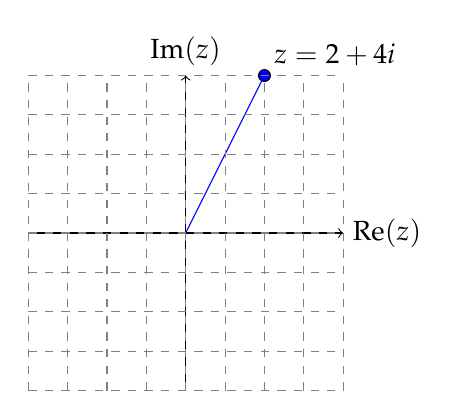
\begin{tikzpicture}[scale=0.5]
                \draw[->] (-4,0) -- (4,0) node[right] {$\Re(z)$};
                \draw[->] (0,-4) -- (0,4) node[above] {$\Im(z)$};
                \draw[fill=blue] (2,4) circle (0.15) node[above right] {$z = 2 + 4i$};
                \draw[-, blue] (0,0) -- (2,4);
                % grid
                \draw[gray, dashed] (-4,-4) grid (4,4);
            \end{tikzpicture}
        \end{center}

        \end{minipage}

        % \vspace{1em}

        % We can actually extend the notion of polar coordinates to complex numbers. If we treat the current $z=a+bi$ form of a complex number as its representation in Euclidean/reectangular coordinates, we can express it in polar form as
        % \[
        % z = r\cos(\theta) + r\sin(\theta)i = r\left(\cos(\theta) + i \sin(\theta)\right)
        % \]
        % where $r = |z|$ and $\theta = \tan^{-1}\left(\frac{b}{a}\right)$. This is known as the \textbf{polar form} of a complex number.
   

    % \begin{tcolorbox}[arc=2mm, colback=magenta!15!white, colframe=magenta!80!black, title=\textsc{Complex Numbers (Enrichment)}]
    %     If you're also familiar with Taylor series, you can show that any complex number can be written as
    %     \[
    %     z = r\left(\cos(\theta) + i\sin(\theta)\right) = r e^{i\theta},
    %     \]
    %     where $e^{i\theta}$ is known as \textbf{Euler's formula}. This formula is particularly useful in PHYS101, where you explore quantum mechanics in more depth.
    % \end{tcolorbox}

    % The number of entries in the ket and bra are determined by how many physical observables are possible in a given physical system. For instance, if we wanted to find the electron's spin in the $z$-direction, we can either be spin up or down, resulting in a two-dimensional bra or ket. 

    \vspace{1em}

    Now that we have established the nature of bras and kets, we can now introduce the \textbf{inner product} of two vectors. In regular Euclidean space, the inner product of two vectors is the dot product, as highlighted above. However, with complex numbers, the inner product is slightly different, and is given the name \textbf{Hermitian inner product}. The Hermitian inner product of two vectors $\bra{\psi}$ and $\ket{\phi}$ is given by
    \[
    \text{For }\bra{\psi} = \begin{bmatrix}
    \psi_1^* &
    \psi_2^* &
    \cdots
    \end{bmatrix}
    \text{ and }\ket{\phi} = \begin{bmatrix}
    \phi_1 \\
    \phi_2 \\
    \vdots
    \end{bmatrix},\quad 
    \braket{\psi}{\phi} = \sum_i \psi_i^* \phi_i.
    \]
    You may notice that if we reverse the order of the vectors, we have
    \[
    \braket{\phi}{\psi} = \sum_i \phi_i^* \psi_i = \left(\sum_i \psi_i^* \phi_i\right)^* = \braket{\psi}{\phi}^*.
    \]
    This is a property unique to the Hermitian inner product: the regular (Euclidean) inner product does not have this property, since all real numbers satisfy $a = a^*$.
\end{tcolorbox}

    \begin{tcolorbox}[arc=2mm, colback=magenta!15!white, colframe=magenta!80!black, title=\textsc{An Introduction to Complex Numbers (Enrichment)}]

    As outlined in Q7.3, there are a couple more properties and vocabulary to take note of. If we take the inner product of a q-vector with itself, we get 
    \[
    \braket{\psi}{\psi} = \sum_i \psi_i^* \psi_i = \sum_i |\psi_i|^2.
    \]
    This looks a lot like the \textit{square} of the magnitude of the q-vector. Indeed! It turns out that the inner product of a q-vector with itself is equal to the square of the q-vector's magnitude.

    \vspace{1em}

    Also recall that the angle between two vectors can be found using the dot product for the Euclidean case. Using this as a heuristic, we see that if $\theta=\pi / 2$, the dot product must be zero, since $\cos(\pi / 2)=0$. This translates to the vectors being perpendicular, or more generally, \textbf{orthogonal} to each other. In the context of quantum mechanics, we say that two vectors are orthogonal if their (Hermitian) inner product is zero.

    \begin{tcolorbox}[colframe=blue!50!black, arc=2mm, title=\textsc{Practice 3}]
        Consider the two q-vectors $\ket{\psi} = \begin{bmatrix} 1+i \\ -1 \end{bmatrix}$ and $\ket{\phi} = \begin{bmatrix} 1+i \\ 2 \end{bmatrix}$. Are they orthogonal?
    \end{tcolorbox}

    \end{tcolorbox}
\end{document}